\documentclass{article}
\usepackage[utf8]{inputenc}
\usepackage[T1]{fontenc} % das Trennen der Umlaute
\usepackage[ngerman]{babel}
\usepackage{colortbl}
\usepackage{microtype}
\usepackage{graphicx}
\usepackage{grffile}
\usepackage{siunitx}  % für Einheiten
\usepackage{hyperref}
\usepackage{amsmath}
\sisetup{locale = DE,  
	separate-uncertainty,  
	range-units = brackets,  
	list-units = single,  
	per-mode=symbol-or-fraction} 
%\usepackage{subfig}
\usepackage{wrapfig}
\usepackage{tikz}
\usetikzlibrary{shapes}
\usepackage{xspace}

%-----------------------------------------------------------------------
%	BIBLIOGRAPHY
%-----------------------------------------------------------------------
\usepackage[style=numeric,sorting=none,backend=biber]{biblatex}
\addbibresource{Bibliographiedatei.bib}
%-----------------------------------------------------------------------


\graphicspath{{Figures/}}

\setlength{\parindent}{0em} 

\title{Dokumentation des BitConnector v5Xe}
\author{Michael Krause \\CC BY-SA 4.0 }

\date{\today}


\begin{document}
\maketitle
%\begin{figure}[!h]
%	\centering
%	\includegraphics[scale=0.06]{Logo}
%\end{figure}

%\thispagestyle{empty}
%\setlength{\unitlength}{1mm}
\begin{picture}(0,0)
\put(230,20){\includegraphics[scale=0.10]{Logo}}
\end{picture} %

\section{Einführung}
Die noch immer andauernden Bemühungen der mikrokosmischen Minimierung von integriertern Schaltkreisen hat Integrationsdichten hervorgebracht, die traditionelle Schaltkreise wie einzelne Register, Zähler, ALUs oder Multiplexer vom Markt verschwinden ließen. Aus der Sicht des Endkonsumentenmarktes mag dieser Schritt folgerichtig sein, jedoch gibt es jenseits dessen noch immer das Bedürfnis auf der Register-Transfer Ebene oder darunter, Logikschaltkreise zu modellieren und zu realisieren. Dieses Bedürfnis kann beispielsweise der akademischen Lehre, dem Wunsch nach Parallelisierung oder der Vorgabe zeitkritischer Anwendungen entspringen. Obwohl es diesbezüglich eine Vielzahl von FPGAs und CPLD-Typen zur Abhilfe gibt, gestaltet sich der prototypische Aufbau auf einem Steckbrett mit Hilfe dieser Chips als nahezu unmöglich. Derartige Chips besitzen meist eine Vielzahl an Pins, die nicht im Dual in-line package (DIP) vorliegen. Der BitConnector versucht dieses Problem zu lösen.

\vspace{0.5cm}

%%Freiheitsgrade ....

\begin{wrapfigure}[14]{l}{0.50\textwidth}
		\vspace { -15pt }
	\includegraphics[scale=0.3]{BitConnector_Overview} 
	\caption{BitConnector v5Xe}
	\label{fig:}
\end{wrapfigure}

Der BitConnector ist ein \textbf{C}omplex \textbf{P}rogrammable \textbf{L}ogic \textbf{D}evice, kurz \textbf{CPLD} Board, das für den  hardwarebasierten, digitalen Prototypenentwurf auf einem Steckboard optimiert wurde und zudem gesockelt auf andere Platinen aufgesetzt werden kann. Das Board ist so entworfen, dass es einen klassischen DIP Chip mit 2,54 mm Rastermaß und 2 * 20 Pins nachbildet. Konfigurationen, die etwa in einer HDL vorliegen, werden mittels JTAG übertragen und dauerhaft auf dem CPLD gespeichert.
 

\section{Eckdaten} 

BitConnector Board-Spezifikation
\begin{itemize}
	\item \textit{Anzahl der frei beschaltbaren Ein/Ausgänge:} \hspace{0.3cm} 33 GPIOs\footnote{\textbf{GPIO}=General Purpose In/Output, \textbf{GRS}=Global Reset, \textbf{GTS}=Global Tri-State, \textbf{GCK}=Global Clock, \textbf{TDI}=Test Data In, \textbf{TDO}=Test Data Out, \textbf{TCK}=Test Clk, \textbf{TMS}=Test Mode Select, \textbf{V\textsubscript{INT}}=Supply voltage internal logic, \textbf{V\textsubscript{IO}}=Supply voltage output driver} und ein Taster
	\item \textit{Gesamtanzahl der Pins:} \hspace{3.6cm} 2 Reihen * 20 Pins (2,54mm)
	\item \textit{kompatible CPLD-Varianten}: \hspace{2.8cm} XC95\textbf{72}XL sowie XC95\textbf{36}XL
	\item Max. Produktterme: \hspace{4.1cm} 1600 bei 72XL/800 bei~36XL
	\item \textit{IC-Package}: \hspace{5.3cm} VQ44 
\end{itemize}

Absolute, maximale Belastbarkeit:
\begin{itemize}
	\item \textit{Versorgungsspannung bezogen auf GND:} \hspace{1cm} -0,5V bis 4V
	\item \textit{IO-Pin Eingangsspannung bezogen auf GND:} \hspace{0.25cm} -0,5V bis 5,5V
	\item \textit{Max. Stromfluss bei max. 70 \si{\celsius} Chiptemp.}:\hspace{0.6cm} $\approx1,6A$ (siehe Kapitel \ref{sec:max_I})
\end{itemize}

Es wird empfohlen, Spannungen über und unter 3,3V($\pm 0,3V$) zu vermeiden!

\section{Pinbelegung BitConnector v5Xe}
\label{sec:Pins}

\begin{minipage}{0.54\textwidth}
	%\begin{table}[h]
	\begin{tabular}{c|c|c}
		DIP-links & CPLD Pin & Funktion\\
		\rowcolor[gray]{.8}	1 & 1 &	GPIO\footnotemark[1], GCK3\footnotemark[1]\\
		2 & 2 & GPIO\footnotemark[1]\\
		\rowcolor[gray]{.8}	3 & 3 & GPIO\footnotemark[1]\\
		4 & 5 & GPIO\footnotemark[1]\\
		\rowcolor[gray]{.8}	5 & 6 & GPIO\footnotemark[1]\\
		6 & 7 & GPIO\footnotemark[1]\\
		\rowcolor[gray]{.8}	7 & 8 & GPIO\footnotemark[1]\\
		8 & 12 & GPIO\footnotemark[1]\\
		\rowcolor[gray]{.8}	9 & 13 & GPIO\footnotemark[1]\\
		10 & 14 & GPIO\footnotemark[1]\\
		\rowcolor[gray]{.8}	11 & 16 & GPIO\footnotemark[1]\\
		12 &  18 & GPIO\footnotemark[1]\\
		\rowcolor[gray]{.8}	13 & 19 & GPIO\footnotemark[1]\\
		14 & 20 & GPIO\footnotemark[1]\\
		\rowcolor[gray]{.8}	15 & 21 & GPIO\footnotemark[1]\\
		16 & 22 & GPIO\footnotemark[1]\\
		\rowcolor[gray]{.8}	17 & 23 & GPIO\footnotemark[1]\\
		18 & 11 & TCK\footnotemark[1] JTAG\\
		\rowcolor[gray]{.8}	19 & 24 & TDO\footnotemark[1] JTAG\\	
		20 & 17,25,4 & GND
	\end{tabular}
	%\end{table}
\end{minipage}
\begin{minipage}{0.2\textwidth}
	\begin{tabular}{||c|c|c}
		DIP-rechts	& CPLD-Pin & Funktion\\
		\rowcolor[gray]{.8}	1		& 15,35 & 3V3/V\textsubscript{INT}\footnotemark[1] \\
		2		& 26 & 		V\textsubscript{IO}\footnotemark[1]\\
		\rowcolor[gray]{.8}	3	& 44 & GPIO, GCK2\footnotemark[1]\\
		4	& 43 & GPIO\footnotemark[1], GCK1\footnotemark[1]\\
		\rowcolor[gray]{.8}	5	& 42 & GPIO\footnotemark[1]\\
		6	& 41 & GPIO\footnotemark[1]\\
		\rowcolor[gray]{.8}	7	& 40 & GPIO\footnotemark[1]\\
		8	& 39 & GPIO\footnotemark[1]\\
		\rowcolor[gray]{.8}	9	& 38 & GPIO\footnotemark[1]\\
		10	& 37 & GPIO\footnotemark[1]\\
		\rowcolor[gray]{.8}	11	& 36 & GPIO\footnotemark[1], GTS1\footnotemark[1]\\
		12	& 34 & GPIO\footnotemark[1], GTS2\footnotemark[1]\\
		\rowcolor[gray]{.8}	13	& 32 & GPIO\footnotemark[1]\\
		14	& 31 & GPIO\footnotemark[1]\\
		\rowcolor[gray]{.8}	15	& 30 & GPIO\footnotemark[1]\\
		16	& 29 & GPIO\footnotemark[1]\\
		\rowcolor[gray]{.8}	17	& 28 & GPIO\footnotemark[1]\\
		18	& 27 & GPIO\footnotemark[1]\\
		\rowcolor[gray]{.8}	19		& 9 & TDI\footnotemark[1] JTAG\\	
		20		& 10 & TMS\footnotemark[1] JTAG
	\end{tabular}
\end{minipage}\\
\begin{minipage}{0.2\textwidth}
	\begin{tabular}{c|c|c}
		\rowcolor[gray]{.8} Taster \hphantom{\hspace*{0.38cm}} & \hphantom{\hspace*{0.55cm}} 33 \hphantom{\hspace*{0.5cm}} &  GRS, high active mit hardware debouncing, sonst low active
	\end{tabular}
\end{minipage}
\newpage




\section{Strom und Spannungsversorgung}

\subsection{Spannungsversorgnung V\textsubscript{ccINT}}
Wie bei traditionellen ICs auch, befindet sich die Betriebsspannung (V\textsubscript{ccINT}) des BitConnectors oben rechts  in Bezug zu GND (unten links).
Auf der Platine ist der V\textsubscript{ccINT} Pin mit „3V3“ beschriftet.
\\\\
\fbox{\parbox[c][0.5cm]{12cm}{V\textsubscript{ccINT} sollte 3.6V nicht übersteigen und 3V nicht unterschreiten. \autocite[3]{XC95_Spec}}}
\\\\
Der BitConnector besitzt aus Gründen der Flexibilität keinen Spannungsregler, es ist daher ratsam die Spezifikationen immer im Auge zu behalten. Ein weitere Fehlerquelle bezüglich {V\textsubscript{ccINT} ist eine unstabilisierten oder unsaubere Spannungsversorgung. In einem solchen Fall wird ein undefiniertes Verhalten bei getakteten/sequenziellen Schaltkreiskonfigurationen zu beobachten sein. 

\begin{figure}[!h]
	\begin{minipage}[!b]{.43\linewidth} % [b] => Ausrichtung an \caption
		\includegraphics[width=\linewidth]{Board_Vcc_incorrect}
		\caption{ungünstige Anbindung an die Versorgungsspannung}
		\label{fig:VCC_fail}
	\end{minipage}
	\hspace{.1\linewidth}% Abstand zwischen Bilder
	\begin{minipage}[!b]{.45\linewidth} % [b] => Ausrichtung an \caption
		\includegraphics[width=\linewidth]{Board_Vcc_correct}
		\caption{empfohlene Anbindung an die Versorgungsspannung}
		\label{fig:VCC_ok}
	\end{minipage}
\end{figure}

Obwohl ich nach der Xilinx Empfehlung \autocite{JTAG_Checklist} Bypass-Kondensatoren für verschiedene Frequenzbereiche auf dem BitConnector vorgesehen habe, um undefiniertem Verhalten vorzubeugen, sollten Sie immer einen zusätzlichen 100nF Kondensator direkt am 3V3 Pin des BitConnectors einsetzen (siehe Abbildung \ref{fig:VCC_ok}). Auch unnötig lange Kabel wie in Abbildung \ref{fig:VCC_fail}) sollten nach Möglichkeit vermieden werden.
%An dieser Stelle ist noch erwähnenswert, dass Sie nach \autocite[17]{XC95_maxI} einen „ stromlosen“ I/O-Pin mit einer maximalen Spannung von V\textsubscript{ccINT}+4V treiben dürfen.

\subsection{Definition der I/O Spannung über V\textsubscript{ccIO}}

Neben der Versorgungsspannung V\textsubscript{ccINT} existiert direkt darunterliegend der Pin V\textsubscript{ccIO}(siehe Kapitel \ref{sec:Pins}), welcher die Höhe der Pin-Ausgangsspannung definiert. Der V\textsubscript{ccIO} Pin ist auf der Platine mit „Vcc“ beschriftet. Sie können die Ausgangsspannung eines Pins in den Bereich zwischen 3,3V bis 2,5V über  V\textsubscript{ccIO} festlegen. Für eine Ausgangsspannung von 3,3 Volt sollte V\textsubscript{ccIO} zwischen 3V und 3,6V liegen. Wird dagegen eine Ausgangsspannung von 2,5V forciert, sollte V\textsubscript{ccIO} zwischen 2,3V und 2,7V liegen, siehe \autocite[3]{XC95_Spec}. Auf diese Weise kann die Ausgangsspannung aller Pins unabhängig von der Versorgungsspannung V\textsubscript{ccINT} eingestellt werden.

\subsection{Ausgangskennlinie eines XC9536XL CPLDs}
Sobald Sie einen GPIO-Pin des BitConnectors als Ausgang definieren und diesen mit einem Stromfluss belasten, in dem Sie beispielsweise eine LED ansteuern, sackt die Ausgangsspannung des entsprechenden Pins ab. Dieser Effekt geht auf den verwendeten CPLD zurück. Um eine Vorstellung zu erhalten, wie sich der treibende Strom zur Spannung verhält, habe ich einige stichpunktartig Messungen durchgeführt. Diese Messwerte sind in Abbildung \ref{fig:out_characteristics} mittels Bezierinterpolation zusammen gefasst und grafisch dargestellt.
Die Messreihe wurde über ein Fluke 87 III auf Pin 37 strom-/spannungsrichtig aufgenommen, V\textsubscript{ccINT} und V\textsubscript{ccIO} betrugen 3,3V. Obwohl es sich bei der Messung um einen XC9536XL CPLD handelt, ist es naheliegend, dass der XC9572XL eine sehr ähnliche Charakteristik zeigt. Verwunderlich ist, dass die Messreihe im Bereich zwischen 2V und 0V eine signifikant Abweichung (max. 10mA bei 0V) von der Xilinx-Spezifikation \autocite[6]{XC_Curves} aufweist.

\begin{figure}[!h]
	\centering
	\includegraphics[width=0.76\linewidth]{Figures/XC9536_output_characteristics}
	\caption{Ausgangskennlinie eines XC9536XL}
	\label{fig:out_characteristics}
\end{figure}

\subsection{Maximaler Stromfluss $I_{max}$}
\label{sec:max_I}
Wer nach einem konkreten Wert bezüglich der maximal zulässigen Stromaufnahme im Datenblatt \autocite{XC95_Spec} des XC95\textbf{72}XL oder des XC95\textbf{36}XL sucht, wird keine derartige Angabe finden.
Zwar wird eine Abschätzung der zu erwartenden Stromaufnahme über eine Formel angegeben, welche die Frequenz, Anzahl der verwendeter Macrozellen u.s.w. mit einbezieht, jedoch bleibt ein maximal zulässiger Stromfluss $I_{max}$ unerwähnt. Der Hauptgrund dafür dürfte wohl an der variablen Umgebungstemperatur und in der individuell eingesetzten Kühlung des ICs liegen. Eine plausible Annahme für derartige Werte und die damit einhergehende maximale Stromaufnahme wäre von Xilinx an dieser Stelle jedoch angebracht gewesen und sei es nur, um eine erste Abschätzung zu bekommen.\\

Um eine solche Abschätzung der maximalen Stromaufnahme $I_{max}$ soll es nachfolgend gehen. Die Berechnung ist ein wenig müßig und führt über verschiedene Dokumentationen.
Zuerst wird die zu $I_{max}$ zugehörige Verlustleistung $P_d$ über folgende Ungleichung berechnet.\autocite[16]{XC95_maxI}: 
\begin{center}
	$T_{jmax} < (\Theta_{JC}*P_d)+T_a$
\end{center}

kurze Variablenbeschreibung:

\begin{itemize}
	\item $T_{jmax}$: Maximaltemperatur in \si{\celsius} bezogen auf das IC Package \\(70 \si{\celsius} für Kunststoff) \autocite[54]{Device_pkg}
	\item $\Theta_{JC}$: Wärmeflusswiderstand in $\si{\celsius}/[W]$ zwischen der Chipoberfläche und der Oberfläche des Gehäuses \autocite[53]{Device_pkg} (8.2 \si{\celsius}/W für 72/36 in VQ44)
	\item $P_d$: tatsächliche Leistung in [W]att, welche sich in Hitze äußert \autocite[16]{XC95_maxI}
	\item $T_a$: Umgebungstemperatur in \si{\celsius} (50 \si{\celsius})
\end{itemize}

Um $\Theta_{JC}$ nicht aufwendig durch eine Messung bestimmen zu müssen, bietet Xilinx eine Datenbank an \autocite{ThetaJC}. Für den XC95\textbf{72}XL/XC95\textbf{36}XL liegt dieser Wert bei 8.2 \si{\celsius}/W im VQ44 Package.\\\\
Zudem schlägt Xilinx für $T_{jmax}$ einen Wert von 70 \si{\celsius} für Kunststoffgehäuse vor. Dieser Wert ist ebenfalls für beide möglichen Chipvarianten angebracht.\\\\
Die Umgebungstemperatur des Chips wird vorsichtig mit 50 \si{\celsius} veranschlagt.\\\\
Ausgehend von diesen Annahmen berechnet sich die Verlustleistung nach \autocite[16]{XC95_maxI} wie folgt:

\begin{center}
	$70 \si{\celsius} = (8.2 \si{\celsius}/W*P_d)+50 \si{\celsius} \Rightarrow$\\
	$20 \si{\celsius} = (8.2 \si{\celsius}/W*P_d)\Rightarrow$\\
	$2,439 W = P_d$\\ %\vspace{0.5cm}
\end{center}

Weiter ist notwendig, die Verlustleistung in $P_d = P_{ddesign} + P_{dIO}$ aufzuschlüsseln.
$P_{ddesign}$ repräsentiert hierbei die Leistung ohne eine Last, also die Leistung die der Chip selbst für sich beansprucht, ohne einen Ausgang zu treiben. Dieser Wert sollte gemessen werden und lautet für den BitConnector rund 40mW. Wird dieser Wert aus Sicherheitsgründen verdoppelt, ist von rund 80mW auszugehen.\\\\
Somit gilt: 
\begin{center}
	$2,439 W = 80mW + P_{dIO}$
\end{center}

Um schlussendlich auf den gesuchten Wert $I_{max}$ zu kommen, wird folgende Formel nach \autocite[16]{XC95_maxI} herangezogen:

\begin{center}
	$I_{max} * (VCC - 1,85V) = P_d - P_{ddesign}$
\end{center}

Sicher fragen Sie sich, woher die 1,85V herstammen. Dieser Wert wurde über die Kennlinienfelder in \autocite[6]{XC_Curves} abgelesen und sagt aus, dass bei einem Stromfluss von 30mA, die Spannung des entsprechenden Ausgangs auf 1,85V absinkt.

Daraus folgt: 
\begin{center}
	$I_{max} * (3,3V - 1,85V) = 2,439 W - 0.08W \rightarrow$\\
	\underline{\underline{$I_{max}\approx 1,63A $}}
\end{center}
Der Wert $I_{max}$ sagt aus, dass bei einer I/O-Spannung von 1,85V und einer Stromstärke von 30mA pro Ausgang, eine Gesamtstromstärke von 1,63A erreicht wird. Hierbei liegt die Chiptemperatur $\leq $ der als kritisch angenommenen 70$\si{\celsius}$. Auffällig ist, dass die 1,63A in dieser Konstellation im Bitconnector nie erreicht werden können, da dieser nur 34 mögliche Ausgänge bietet. Mit den getroffenen Annahmen ist jedoch die Versorgung von $\frac{1,63A}{0,03A}\approx54$ Ausgänge möglich.\\\\
Bitte verlassen Sie sich nicht auf die angegebene Berechnung und überprüfen Sie auch die Quellen. Sollten Sie einen Fehler finden, wäre ich Ihnen sehr dankbar, wenn Sie mich diesbezüglich kontaktieren.

\newpage

\section{Hardware Entprellung}
Gelegentlich ist es sehr hilfreich, eine getaktete, sequenzielle Schaltung schrittweise über das Drücken eines Taster zu durchlaufen. Leider erzeugen so ziemlich alle handelsüblichen Taster ein sogenanntes „Prellen“, da die Kontakte des Tasters nicht sauber schließen oder öffnen. Ein solches Prellen führt zu einer unvorhersagbaren Abfolge von Signalimpulsen. Schauen Sie sich hierfür einmal die Abbildung \ref{fig:prellen_1} genauer an. 

\begin{figure}[!h]
	\centering
	\includegraphics[width=0.92\linewidth]{Figures/bounce}
	\caption{Tastendruck am BitConnector ohne Entprellung}
	\label{fig:prellen_1}
\end{figure}

Hier wird ein einfacher Tastendruck über ein Oszillogramm grafisch veranschaulicht. Interessant ist der Bereich der fallende Flanke ab 80 Millisekunden, also ungefähr an der Stelle, an dem der Taster wieder losgelassen wird. Wenn Sie diesen Bereich kritisch betrachten, werden Sie bemerken, dass es bei ungefähr 92 Millisekunden bereits einen ungewollten Wechsel der Signalflanke gibt. Lassen Sie uns diesen Bereich mit der „Lupe“ in Abbildung \ref{fig:prellen_2} etwas näher betrachten.

\begin{figure}[!h]
	\centering
	\includegraphics[width=0.92\linewidth]{Figures/bounce_near}
	\caption{Nahaufnahme der fallenden Flanke aus Abbildung \ref{fig:prellen_1}}
	\label{fig:prellen_2}
\end{figure}

Es ist erkennbar, dass der Signalpegel in Abbildung \ref{fig:prellen_2} bereits bei ungefähr 2 Millisekunden hin und herspringt und somit mehrere Flanken erzeugt. Diese Signalflanken sind bei sogenannten sequenziellen Schaltungen, die auf fallende oder steigende Flanken reagieren, problematisch. Eine einfache Zählerschaltung, die mit jedem Tastendruck „1“ hinzu addiert, wird augenscheinlich nicht funktionieren. So scheint es, als würde der Zähler einzelne Zählschritte beim Drücken oder Loslassen des Tasters überspringen. Mit einem höherwertigen Oszilloskop ließe sich der problematische Bereich noch näher untersuchen, was weitere Taktwechsel und somit weitere Zählimpulse mit nur einem Tastendruck aufdecken könnte. 
Da Sie bei CPLDs prinzipiell mit Ihren Flip-Flop-Ressourcen sehr haushalten müssen und keinen Mikrocontroller für eine Entprellroutine haben, wurde für den BitConnector eine Hardwareentprellung vorgesehen. 

\newpage

Sollte Ihr BitConnector mit dem 74LVC2G14 IC bestückt sein, so ist auch der Taster SW1 automatisch entprellt. Ein Tastendruck sollte dann wie in Abbildung \ref{fig:prellen_3} eine einzige und saubere Flanke erzeugen. 


\begin{figure}[!h]
	\centering
	\includegraphics[width=0.92\linewidth]{Figures/debounce}
	\caption{Tastendruck am BitConnector mit Hardware-Entprellung}
	\label{fig:prellen_3}
\end{figure}

Sollte dies nicht der Fall sein, so können Sie auf Grundlage der nachfolgenden Erläuterungen eine eigene Hardwareentprellung nachschalten.

\subsection{Prinzip der Hardwareentprellung}
Da die vom Menschen erzeugten Frequenzen der Tastendrücke im Vergleich zum Prellen des Tasters sehr niedrig sind, ist es naheliegend einen Tiefpassfilter in Form eines RC-Gliedes dem Taster vorzuschalten. 
Dieser Tiefpass filtert die hochfrequenten Anteile des Prellens aus dem Tastendruck heraus. Das Prellen ist verschwunden. Es entsteht allerdings ein neues Problem. Da ein RC-Glied naturgemäß aus einem Widerstand und einem Kondensator besteht, durchläuft dieser Kondensator eine Ladespannung, die dem natürlichen Logarithmus sehr nahe kommt \autocite{RC}. Eine digitale Schaltung auf CMOS-Basis benötigt jedoch eine steile Signalflanke, also beispielsweise einen Signalwechsel von 0V auf direkt 3,3V. Andernfalls besteht die Gefahr, dass die Schaltung eine gewisse Zeit einen undefinierten Zustand annimmt. Auf Transistorebene kann dieser undefinierte Zustand gefährlich sein, da eine Transistorkonstellation, die es theoretisch so nicht geben sollte, plötzlich anfangen kann, den Strom zu leiten. Zudem werden Sie immer noch keine Freude beim auswerten des Tastenimpuls haben. Es ist daher nachdrücklich anzuraten, diese undefinierten Signalzustände in digitalen Schaltungen zu vermeiden. Dies geschieht hier mit Hilfe eines Schmitt-Triggers. Der Schmitt-Trigger soll verkürzt dargestellt, den undefinierten Spannungsbereich vor dem digitalen Eingang einer Schaltung über eine sogenannte „charakteristische Hysterese“ vermeiden. Sie können sich den Schmitt-Trigger in diesem Fall als den „eigentlichen Schalter“ vorstellen, der an seinem Ausgang immer einen steilen Pegel schaltet, während er am Eingang eine Kondenstorkennlinie „sieht“.
%Grafiken (Auch Schaltplan) und Berechnungen einfügen.


\section{Entwicklungsumgebung}

Momentan gibt es noch keine vollumfängliche und freie \autocite{FSF} Entwicklungsumgebung für Xilinx CPLDs, weshalb ich auf proprietäre Software der Firma Xilinx zurückgreifen muss.
Fraglicherweise bietet Xilinx in seiner aktuellen Entwicklungsumgebung „Vivado“ keine Unterstützung für CPLDs an, siehe \autocite[17]{Vivado}. Dennoch ist es möglich, mit der älteren Design Suite „ISE“, Xilinx CPLDs problemlos zu konfigurieren.
Mit einer Registrierung bei Xilinx erhalten Sie eine kostenlose Lizenz, mit derer Sie die ISE-Demo-Version auf eine Webpack-Version \autocite{ISE-Web} freischalten können. Diese Lizenz ist ausreichend, um alle CPLDs der XC9500 Serie ohne Einschränkungen zu konfigurieren.

\section{Die JTAG Schnittstelle via 6 Pin IDC-Header}

Für die Übertragung der HDL Konfigurationsdateien auf den BitConnector ist ein 6 Pin IDC-Stecker (JTAG Schnittstelle) im 2.54mm Rastermaß vorgesehen. Die 4 aktiven JTAG-Leitungen zur Datenübertragung sind:

\begin{enumerate}
	\item Pin TCK = Test Clock
	\item Pin TDI = Test Data In
	\item Pin TDO = Test Data Out
	\item Pin TMS = Test Mode Select
\end{enumerate}

\begin{figure}[!h]
	\centering
	\includegraphics[width=0.25\linewidth]{Figures/PinHeader6P_male}
	\caption{Draufsicht JTAG Pin-Header (6 way IDC male connector)}
	\label{fig:pinheader}
\end{figure}

\newpage

Die Abbildung \ref{fig:pinheader} zeigt die Draufsicht dieses Steckers, welcher auf dem Board verlötet ist.
Innerhalb dieser Abbildung erkennen Sie eine „1“, die den ersten Pin markiert. Dieser Pin ist zur Orientierung dem JTAG Test-Takt zugeordnet. Um die Anfertigung eines eigenen Programmierkabels zu erleichtern, wird nachfolgend auch das passende Datenkabel illustriert. Ich möchte Sie ermutigen, die Anfertigung eines eigenen Kabels nicht zu fürchten. Die Minimalausrüstung sehen sie in Abbildung \ref{fig:cable_equipment}

\begin{figure}[!h]
	\centering
	\includegraphics[width=1\linewidth]{Figures/cable_equipment}
	\caption{Werkzeug und Ribbon Cable + IDC-Stecker zum selber crimpen}
	\label{fig:cable_equipment}
\end{figure}

Da es mehrere Programmiergerät gibt, existieren somit mehrere Stecker-Möglichkeiten und Adapter.  In Abbildung \ref{fig:data_cable} erkennen Sie ein mögliches Datenkabel vom BitConnector zum Programmiergerät. Anders als in Abbildung \ref{fig:pinheader}, ist der 6 Pin Connector diesmal als Buchse ausgeführt und somit gespiegelt.

\begin{figure}[!h]
	\centering
	\includegraphics[width=0.9\linewidth]{Figures/14Pin_to_6Pin_data_cable}
	\caption{Programmierkabel HW-RIBBON14 zu 6 Pin IDC female}
	\label{fig:data_cable}
\end{figure}

Bei dem HW-RIBBON14 female connector hat sich Xilinx für eine eher exotische Buchse entschieden. Die Kette des Datenkabels sieht abstrakt zusammen gefasst folgendermaßen aus:
\vspace{0.5cm}
\begin{center}
	PC<->USB-Kable<->Programmierer<->Programmierkabel<->BitConnector
\end{center}

\vspace{0.5cm}

\newpage

Falls Sie kein passendes Kabel zur Hand haben, können Sie die herausgeführten JTAG Pins von den beiden Stiftleisten über ein Steckbrett abgreifen(rote Markierung).

\begin{figure}[!h]
	\centering
	\includegraphics[width=0.4\linewidth]{Figures/JTAG_Pins}
	\caption{Die JTAG Schnittstelle, einmal rot umkreist als Stiftleisten und grün umkreist als IDC Header ausgeführt}
	\label{fig:JTAG_Pins}
\end{figure}

Sofern Sie mehrere BitConnectoren auf einer Platine gesockelt haben, bieten sich die Pins der Stiftleisten ebenfalls an, um die CPLDs mit nur einer herausgeführten Schnittstelle sequenziell zu konfigurieren.
\subsection{JTAG Programmiergerät}
Für die Ansteuerung der JTAG-Schnittstelle wird ein Programmiergerät benötigt. 
Hier gibt es mehrere Lösungen mit unterschiedlichen Funktionsumfang. Verbreitet sind 4 Versionen des Xilinx Platform Cable USB I/II. Dabei entfallen bereits 3 Versionen auf das Platform Cable I: 
\begin{itemize}
	\item \textbf{DLC9G} (neuste Version bezüglich Platform Cable I)
	\item \textbf{DLC9LP} (Vorgänger des DLC9G)
	\item \textbf{DLC9} (älteste Version)
\end{itemize}

\newpage

Zu diesen 3 Versionen schreibt Xilinx u.a.: „\textit{The DLC9G and legacy DLC9LP cable models draw less than 100 mA from the host USB port. The legacy DLC9 cable model requires 230 mA to operate in USB 2.0 Hi-Speed mode or 150 mA to operate in USB 2.0/1.1 full-speed mode.}“ \autocite[2]{Platform_Cable}\\\\
Das Xilinx Platform Cable USB II wird momentan unter der Versionsbezeichnung „\textbf{DLC10}“ gehandelt.
Die hohen Verbreitung dieser Programmiergeräte hat dazu beigetragen, dass es selbige auch als preisgünstige Nachbauten von anderen Herstellern zu einem Zehntel des Preises gibt.

\begin{figure}[!h]
	\centering
	\includegraphics[width=1\linewidth]{Figures/JTAG_Programmer_uebersicht}
	\caption{oben: XUP USB-JTAG Programming Cable
		\\\hspace*{2cm} unten: Platform Cable USB II DLC10}
	\label{fig:JTAG_Cable}
\end{figure}

Als Alternative zum „Platform Cable I/II“ existiert eine kleine und günstigere Variante aus dem „Xilinx University Program“ dass die Bezeichnung „XUP USB-JTAG Programming Cable“ trägt. Sie können es nachfolgend in Abbildung \ref{fig:JTAG_Cable} erkennen. Allerdings scheint diese Variante mit dem heutigen Preisverfall des Platform Cables I/II wenig attraktiv zu sein. 
Der Vollständigkeit halber soll an dieser Stelle noch das \textbf{DLC7}/Parallel Cable IV erwähnt werden, dass jedoch in der neuen Entwicklungsumgebung von Xilinx/Vivado nicht mehr unterstützt wird \autocite{AR_54136} und aufgrund der „ausgestorbenen“ parallelen Schnittstelle bei Anwendern ebenfalls nur mehr selten anzutreffen sein dürfte. Wenn Sie keinen Wert auf Zusatzfunktionen wie „SPI PROM Support, ChipScope oder AES-Cryptographic“ legen, sollte die Wahl des Programmers eine untergeordnete Rolle spielen.

\newpage

\subsection{Offene JTAG Hardware-/Softwarelösungen für Xilinx}
Es gibt einige Projekte, die sich darum bemühen, alternative und offene JTAG Hardware-/Softwarelösungen für Xlinix Produkte anzubieten.
Um ein CPLD/FPGA zu konfigurieren, wird ein Mikrocontroller (JTAG-Programmiergerät) benötigt, der den JTAG Standard „IEEE 1149.1“ und eventuelle herstellerspezifische Abweichungen implementiert. 
Um mit diesem Mikrocontroller kommunizieren zu können, wird weiter eine PC-Software (JTAG Client) benötigt, welche die HDL synthetisierte Konfiguration (im XSVF Format) an diesen Mikrocontroller überträgt. Der Mikrocontroller nimmt letztlich über das vom PC aus übertragene XSVF Format die Konfiguration des CPLD/FPGA mittels JTAG vor.

\begin{figure}[!h]
	\centering
	\includegraphics[width=0.8\linewidth]{Figures/iMPACT}
	\caption{Das proprietäre iMPACT überträgt und verifiziert die HDL Konfiguration (über ein JTAG Programmiergerät) auf dem CPLD oder FPGE}
	\label{fig:iMPACT}
\end{figure}

Um aber auf die offenen Alternativen hinzuweisen, soll hier die Lib(X)SVF von Clifford Wolf\autocite{LibXSVF} Erwähnung finden. Lib(X)SVF ist eine C-Bibliothek zur Implementierung/Umsetzung von JTAG-Programmiergeräten mittels XSVF/SVF Format. Eine konkrete Implementierung ist beispielsweise das „clujtag“ Projekt, wobei clujtag \autocite{clujtag} die Firmware eines einfachen AVR basierten Programmiergeräts bildet und clujtag-client \autocite{clujtag-client} eine kommandozeilenbasierte Alternative zu Xilnix iMPACT darstellt.
In welchen Umfang diese und andere Projekte heute tragfähig sind, kann ich bisher nicht einschätzen.


\newpage
\printbibliography
\end{document}